\section{IoTサービスとは}
% (IoTサービスがどのようなもので、どのような背景で登場してきたのか、どんなものがありどのような自動化を図っているのか)}
IoTとは、Internet of Things の略で「モノのインターネット」とも呼ばれる概念である。
IoTでは、様々な物がインターネットにつながり、相互に情報をやり取りすることで、多様な自動化を行う。
IoTサービスとは、ユーザーに対しIoTによる利便性を提供するものである。
\medskip

IoTサービスは、半導体技術の進歩によりコンピューターが小型且つ安価になったこと、通信ネットワークの整備が進み様々な場所から安価に通信が利用可能になったことで登場した。
\medskip

例えば、次のような物がある。
\begin{itemize}
	\item コーヒーポット
	\item 太陽光発電の監視
\end{itemize}

コーヒーポットの自動化とは、コーヒーポットまで移動し、コーヒーポットの状態を確認しに行く手間を省くためのサービスである。
このサービスの実現の為に、コーヒーポットに対してコンピューターを取り付ける。
これらコンピューターが、コーヒー豆の残量やコーヒーが入ったか否かの情報をサーバーとやり取りする。
それにより、サーバーはコーヒー豆の自動発注や、コーヒーが入ったことユーザーに知らせる。
\medskip

太陽光発電の監視とは、太陽光発電所の発電量や機器の異常を確認しに行くための手間を省くためのサービスである。
このサービスの実現の為に、太陽光発電所の機器にコンピューターを取り付ける。
これらコンピュータが発電量や機器の異常の情報をサーバーとやり取りする。
それにより、サーバーは、発電量や機器の異常をユーザーに知らせる。
\medskip

このように、IoTサービスは、IoT機器とサーバーが連携し、ユーザーに利便性を提供するものである。
今後も数多くサービスが登場すると考えられている。

\section{IoTサービスの構造とは}
%(IoTサービスの構造要素としてIoT機器とサーバがあること、IoT機器・サーバーとはどのようなものなのか、何をしているのか、その間の通信とはどのようなものなのか)
IoTサービスは、IoT機器とサーバーが連携し利便性を提供するものである。
IoTサービスの構造として、多数のIoT機器とサーバーがインターネットを介し連携する事が挙げられる。
\medskip

\begin{figure}[htbp]
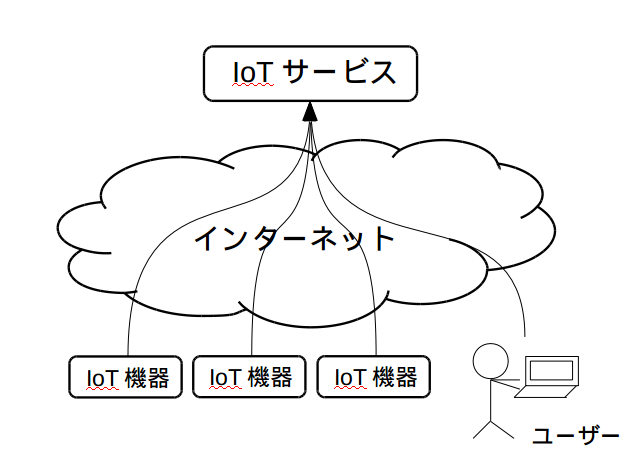
\includegraphics[width=16cm]{images/IoTservice.png}
\caption{IoTサービスの構成図}
\label{fig:IoTservice}
\end{figure}

IoT機器は、様々な環境へ設置され、周囲の状況を検知することや、周囲へなんらかの働きを行う為に使用される。
コーヒーポットの例では、コーヒーが出来上がったか否かを検知する。また、コーヒーポットに対し、コーヒーを入れるよう働きかけている。
\medskip

この機器からの情報を収集し、処理しているのがサーバーである。
サーバーは、IoT機器からの情報を蓄積・分析し、IoT機器やユーザーに対し何らかの働きかけを行う。
コーヒーポットの例では、ユーザーがコーヒーを入れた回数からコーヒー豆の残量を分析し発注を行うよう働きかけている。
\medskip

サーバーにて動作するプログラムが、IoT機器と通信することで、IoTサービスを構成する。
この通信に利用されるのがインターネットである。
様々な通信リンクを用いてIoT機器とサーバー上のプログラムが連携する。
\medskip

このように、IoTサービスの構造は、IoT機器とサーバー上のプログラムがインターネットを介し通信し、連携することで成り立っている。

\section{IoTサービス維持の問題}
%(IoTサービスの維持の為に何が必要となるのか、それを妨げている物はなんなのか)
IoTサービスは、IoT機器とサーバー上のプログラムがインターネットを介し通信し合うことで成り立っている。
IoTサービスを維持するためには、これらの構造を維持する必要がある。
そのため、IoT機器が正常に動作しているのか、通信が途切れていないか、監視する事が重要である。
ところが、IoT機器が多量に存在することや、IoT機器が接続するネットワークが多様であることから、その監視には技術的困難がある。
また、個別のIoTサービスに組み込まれた監視システム等を別として、一般的な監視サービスも存在しない。
\medskip

IoTサービスでは、多量のIoT機器を使用する。
そのため、個々のIoT機器を識別し、適切に管理することが困難である。
\medskip

また、家庭内や屋外等、様々な環境下に置かれるIoT機器が接続されるネットワークを予め予期することは困難を極める。
接続先のネットワークでもプライベートアドレスを付与されるなどの他、IoT機器とサーバーとの通信に制限がかかる場合もある。
さらに、IoT機器によっては、移動することを前提とした物もある。
そのような場合、接続されるネットワークが頻繁に切り替わりるため、既存の機器のIPアドレスを利用した機器監視手法は適応することができない。
そのため、遠隔から機器の状態を確認することが難しい。
\medskip

このように、IoTサービスの維持において、IoT機器の動作や通信状態を監視することは重要であるが、その監視には技術的な困難がある。
IoTサービスの円滑な提供や今後の発展の為には、技術的な困難を越えたIoT機器の監視の実現が重要である。


\section{従来の機器監視手法の適応}
ここで従来の機器監視手法を上げてみる。
\subsection{SNMPを用いた機器の監視}
	SNMPとは、SimpleNetworkManagementProtocolの略で、ネットワーク機器を監視するために作られた。
	監視対象機器で動作するSNMPエージェントと、監視用機器で動作するSNMPマネージャーからなる。
	しかしセキュリティの観点からネットワーク機器にてブロックされることがある。
	また、見かけのIPアドレスと、SNMPが持つIPアドレスが違うと、混乱する場合がある。
	また、監視用機器側で、監視対象IPアドレスを記憶しておく必要がある。
	機器のIPアドレスが頻繁に変わる事を考えると、現実的ではない。
\subsection{Pingを用いた機器の監視}
	Pingとは、ICMPを利用したプログラムで、監視対象機器へICMPEchoRequestというメッセージを送信し、
	監視対象機器は、ICMPEchoReplyというメッセージを返すことで、機器の動作状態や、ネットワークへの接続性を確認するプログラムである。
	これも同様に、監視用機器側で、監視対象IPアドレスを記憶しておく必要があるため、IoT機器の監視には向かない。
	セキュリティの観点からネットワーク機器にてブロックされることが多い。
\subsection{Logstash・Elasticksearch・Kibanaを用いた機器の監視}
	Logstashとは、機器の状態を収集し転送するプログラムである。
	監視対象機器と監視機器双方で動作している必要がある。
	Elasticksearchとは、機器の状態を蓄積するデータベースである。
	Kibanaはデータベース内の機器の状態を可視化するプログラムである。
	これら三つが連携することで機器の監視を行う解決策がある。
	しかし、IoT機器の上でLogstashが動作する必要がある。
	また、各IoT機器にインストールされたLogstashと、機器監視サーバ上で動作するElasticksearchやKibanaを適切に設定する必要がある。
	IoT機器が追加される度に、新たにKibanaに対し設定をしなければならないので、手間がかかる。
\subsection{Teregraf・Influxdb・Grafanaを用いた機器の監視}
	Teregrafとは、機器の状態を収集し転送するプログラムである。
	Influxdbは、機器の状態を時系列に整理し格納するデータベースである。
	そのデータベースの可視化プログラムとして、Grafanaがある。
	しかし、この組み合わせも、上記Logstash・Elasticksearch・Kibanaの時と同様に各ソフトウェアに適切な設定が必要であり、
	IoT機器が追加される度にGrafana上で追加の設定をシなければならない。

